\documentclass[11pt]{article}

\usepackage[margin=1in]{geometry}
\usepackage{amsmath, amssymb}
\usepackage{mathtools}
\usepackage{enumitem}
\usepackage{parskip}
\usepackage{graphicx}
\usepackage{booktabs}
\usepackage{array}
\usepackage{listings}
\usepackage{xcolor}

\title{A-7A Corsair II Stability and Control Analysis \\
       \large AERO 321 Final Project}
\author{}
\date{}

\newcommand{\qbar}{\bar{q}}
\newcommand{\cbar}{\bar{c}}
\newcommand{\Ixx}{I_{xx}}
\newcommand{\Iyy}{I_{yy}}
\newcommand{\Izz}{I_{zz}}
\newcommand{\Ixz}{I_{xz}}
\newcommand{\dd}[2]{\dfrac{\partial #1}{\partial #2}}

\lstdefinestyle{pythonstyle}{
    language=Python,
    basicstyle=\ttfamily\footnotesize,
    keywordstyle=\color{blue!70!black},
    commentstyle=\color{green!40!black}\itshape,
    stringstyle=\color{red!60!black},
    numbers=left,
    numberstyle=\tiny\color{gray},
    numbersep=8pt,
    breaklines=true,
    breakatwhitespace=true,
    showstringspaces=false,
    frame=single,
    rulecolor=\color{gray!50},
    columns=fullflexible,
    keepspaces=true,
    tabsize=4,
}

\begin{document}
\maketitle

\section*{Introduction}
\addcontentsline{toc}{section}{Introduction}

placeholder

\part*{Longitudinal Stability Derivatives}
\addcontentsline{toc}{part}{Longitudinal Stability Derivatives}

\section{Longitudinal Nondimensionalization Conventions}

Dimensional derivatives are obtained by differentiating the dimensional aerodynamic
forces and moments with respect to each motion variable, then expressing the result
through the nondimensional coefficients defined as
\begin{equation}
C_X = \frac{X}{\qbar S}, \qquad
C_Z = \frac{Z}{\qbar S}, \qquad
C_m = \frac{M}{\qbar S \cbar},
\end{equation}
together with the nondimensional perturbation variables
\begin{equation}
\hat{u} = \frac{u}{U_1}, \qquad
\hat{\alpha} = \alpha, \qquad
\hat{\dot\alpha} = \frac{\dot\alpha\,\cbar}{2U_1}, \qquad
\hat{q} = \frac{q\cbar}{2U_1}, \qquad
\hat{\delta}_e = \delta_e .
\end{equation}
Derivatives are taken about the trim state (subscript $1$), where $U = U_1$
and $\qbar = \qbar_1 = \tfrac{1}{2}\rho_1 U_1^2$.

\section{X-Force Derivatives}

In stability axes, the total axial force, including the steady contribution and
perturbations, is
\begin{equation}
X = \qbar S\,C_X = \tfrac{1}{2}\rho U^2 S\,(-C_D + C_T),
\end{equation}
where $-C_D$ reflects drag acting opposite to the body $x$-axis and $C_T$ is the
thrust coefficient.

\subsection{Derivative with respect to $u$}

Differentiating with respect to $u$ at trim, recognizing that both $U^2$ and $C_D$
depend on $u$:
\begin{equation}
\dd{X}{u} = \rho_1 U_1 S\,(-C_{D_1}) + \tfrac{1}{2}\rho_1 U_1^2 S\left(-\dd{C_D}{u}\right).
\end{equation}
Using $\hat u = u/U_1$, the chain rule gives $\partial C_D/\partial u = C_{D_u}/U_1$.
Substituting and factoring $\qbar_1 S/(mU_1)$:
\begin{equation}
\boxed{\;X_u = \frac{1}{m}\dd{X}{u} = -\frac{\qbar_1 S}{mU_1}\bigl(C_{D_u} + 2C_{D_1}\bigr)\;}
\end{equation}
The factor of $2$ originates from differentiating $U^2$; $C_{D_u}$ accounts for
compressibility (Mach) effects on drag.

\subsection{Derivative with respect to $\alpha$}

At fixed $U_1$, only $C_D$ and $C_L$ depend on $\alpha$. Resolving forces in the
stability $x$-axis (small-angle: $\sin\alpha \approx \alpha$) gives a contribution
from lift tilting forward:
\begin{equation}
X = \qbar_1 S\,(-C_D + C_L\,\alpha + \cdots).
\end{equation}
Differentiating and evaluating at trim ($\alpha = \alpha_1$, the explicit $\alpha$
factor drops out but $C_{L_1}$ survives the product rule):
\begin{equation}
\boxed{\;X_\alpha = \frac{1}{m}\dd{X}{\alpha} = -\frac{\qbar_1 S}{m}\bigl(C_{D_\alpha} - C_{L_1}\bigr)\;}
\end{equation}

\subsection{Derivative with respect to $\delta_e$}

Only the elevon-induced drag contributes (the elevon-lift contribution to $X$ is
negligible at small $\alpha_1$):
\begin{equation}
\boxed{\;X_{\delta_e} = -\frac{\qbar_1 S}{m}C_{D_{\delta_e}}\;}
\end{equation}

\subsection{Thrust derivative $X_{T_u}$}

By identical reasoning to $X_u$, applied to the thrust term $+C_T$:
\begin{equation}
\boxed{\;X_{T_u} = \frac{\qbar_1 S}{mU_1}\bigl(C_{T_{X_u}} + 2C_{T_{X_1}}\bigr)\;}
\end{equation}

\subsection{Conversion between $\alpha$ and $w$}

Since $w = U_1\sin\alpha \approx U_1\alpha$, the chain rule gives
\begin{equation}
X_w = \dd{(X/m)}{w} = \frac{1}{U_1}\dd{(X/m)}{\alpha}
\quad\Longrightarrow\quad \boxed{\;X_\alpha = U_1 X_w\;}
\end{equation}

\section{Z-Force Derivatives}

The vertical force (with lift acting in $-z$) is
\begin{equation}
Z = -\qbar S\,C_L \quad (\text{plus a small } C_D\sin\alpha \text{ correction}).
\end{equation}

\subsection{Derivative with respect to $u$}

\begin{equation}
\dd{Z}{u} = -\rho_1 U_1 S\,C_{L_1} - \tfrac{1}{2}\rho_1 U_1^2 S\,\frac{C_{L_u}}{U_1},
\end{equation}
\begin{equation}
\boxed{\;Z_u = -\frac{\qbar_1 S}{mU_1}\bigl(C_{L_u} + 2C_{L_1}\bigr)\;}
\end{equation}
The structure mirrors $X_u$, with $C_L$ replacing $C_D$.

\subsection{Derivative with respect to $\alpha$}

The body-axis $Z$-force depends on both $C_L$ and the $\alpha$-projection of $C_D$:
\begin{equation}
Z = -\qbar_1 S\bigl(C_L + C_D\,\alpha\bigr).
\end{equation}
Differentiating with respect to $\alpha$ and evaluating at trim:
\begin{equation}
\boxed{\;Z_\alpha = -\frac{\qbar_1 S}{m}\bigl(C_{L_\alpha} + C_{D_1}\bigr)\;}
\end{equation}

\subsection{Derivatives with respect to $\dot\alpha$ and $q$}

These come from unsteady aerodynamic terms. The nondimensional derivatives use
$\hat{\dot\alpha} = \dot\alpha\,\cbar/(2U_1)$ and $\hat q = q\cbar/(2U_1)$, so
converting back to dimensional $\dot\alpha$ and $q$ introduces a factor $\cbar/(2U_1)$:
\begin{equation}
\boxed{\;Z_{\dot\alpha} = \frac{1}{m}\dd{Z}{\dot\alpha}
       = -\frac{\qbar_1 S\cbar}{2mU_1}C_{L_{\dot\alpha}}\;}
\end{equation}
\begin{equation}
\boxed{\;Z_q = \frac{1}{m}\dd{Z}{q}
       = -\frac{\qbar_1 S\cbar}{2mU_1}C_{L_q}\;}
\end{equation}

\subsection{Derivative with respect to $\delta_e$}

\begin{equation}
\boxed{\;Z_{\delta_e} = -\frac{\qbar_1 S}{m}C_{L_{\delta_e}}\;}
\end{equation}

\subsection{Conversion to $w$-derivatives}

By the same chain rule as for $X$:
\begin{equation}
\boxed{\;Z_\alpha = U_1 Z_w, \qquad Z_{\dot\alpha} = U_1 Z_{\dot w}\;}
\end{equation}

\section{M-Pitching Moment Derivatives}

The pitching moment is $M = \qbar S \cbar\,C_m$, and the dimensional derivative is
$M_{(\cdot)} = (1/\Iyy)\,\partial M/\partial(\cdot)$.

\subsection{Derivative with respect to $u$}

Both $\qbar$ and $C_m$ depend on $u$. Following the same expansion as for $X_u$:
\begin{equation}
\dd{M}{u} = \rho_1 U_1 S\cbar\,C_{m_1} + \qbar_1 S\cbar\,\frac{C_{m_u}}{U_1},
\end{equation}
\begin{equation}
\boxed{\;M_u = \frac{\qbar_1 S\cbar}{\Iyy U_1}\bigl(C_{m_u} + 2C_{m_1}\bigr)\;}
\end{equation}
In trimmed flight $C_{m_1} = 0$, but the formula retains the term for generality.

\subsection{Derivatives with respect to $\alpha$ and $\delta_e$}

These are static (no time scaling needed):
\begin{equation}
\boxed{\;M_\alpha = \frac{\qbar_1 S\cbar}{\Iyy}C_{m_\alpha}\;}
\end{equation}
\begin{equation}
\boxed{\;M_{\delta_e} = \frac{\qbar_1 S\cbar}{\Iyy}C_{m_{\delta_e}}\;}
\end{equation}

\subsection{Derivatives with respect to $\dot\alpha$ and $q$}

Both involve the unsteady-aerodynamic nondimensionalization $\cbar/(2U_1)$.
Importantly, $M$ already carries one factor of $\cbar$ from its own coefficient
definition, so the dimensional derivative ends up with $\cbar^{\,2}$:
\begin{equation}
\boxed{\;M_{\dot\alpha} = \frac{1}{\Iyy}\dd{M}{\dot\alpha}
       = \frac{\qbar_1 S\cbar^{\,2}}{2\Iyy U_1}C_{m_{\dot\alpha}}\;}
\end{equation}
\begin{equation}
\boxed{\;M_q = \frac{1}{\Iyy}\dd{M}{q}
       = \frac{\qbar_1 S\cbar^{\,2}}{2\Iyy U_1}C_{m_q}\;}
\end{equation}

\subsection{Thrust-pitching derivatives}

Same logic as $X_{T_u}$ applied to the moment:
\begin{equation}
\boxed{\;M_{T_u} = \frac{\qbar_1 S\cbar}{\Iyy U_1}\bigl(C_{m_{T_u}} + 2C_{m_{T_1}}\bigr)\;}
\end{equation}
\begin{equation}
\boxed{\;M_{T_\alpha} = \frac{\qbar_1 S\cbar}{\Iyy}C_{m_{T_\alpha}}\;}
\end{equation}

\subsection{Conversion to $w$-derivatives}

\begin{equation}
\boxed{\;M_\alpha = U_1 M_w, \qquad M_{\dot\alpha} = U_1 M_{\dot w}\;}
\end{equation}

\section{Longitudinal Pattern Summary}

Three structural elements appear repeatedly:
\begin{enumerate}[leftmargin=*]
  \item The $+2 C_{(\cdot)_1}$ term in every $u$-derivative comes from differentiating
        $\qbar \propto U^2$ at trim. It is a kinematic effect, present even when the
        coefficient itself has zero Mach sensitivity.
  \item The factor $\cbar/(2U_1)$ appears whenever the nondimensionalization used
        $\hat q$ or $\hat{\dot\alpha}$. Pitching-moment versions carry $\cbar^{\,2}$
        because $M$ contributes its own $\cbar$.
  \item The $\alpha\!\leftrightarrow\!w$ transformation $(\cdot)_\alpha = U_1(\cdot)_w$
        follows directly from $w = U_1\alpha$ at small angles and applies uniformly
        to $X$, $Z$, and $M$.
\end{enumerate}

\part*{Lateral-Directional Stability Derivatives}
\addcontentsline{toc}{part}{Lateral-Directional Stability Derivatives}

\section{Lateral-Directional Nondimensionalization Conventions}

In stability axes, the lateral-directional aerodynamic side force, rolling moment,
and yawing moment are nondimensionalized as
\begin{equation}
C_y = \frac{Y}{\qbar S}, \qquad
C_\ell = \frac{L}{\qbar S b}, \qquad
C_n = \frac{N}{\qbar S b},
\end{equation}
where $L$ denotes the rolling moment (not lift) and $b$ is the wingspan. The key
distinction from the longitudinal case is that the reference length is the
span~$b$ rather than the chord~$\bar c$, because rolling and yawing moments scale
naturally with span.

The lateral-directional perturbation variables are
\begin{equation}
\hat\beta = \beta, \qquad
\hat p = \frac{p\,b}{2U_1}, \qquad
\hat r = \frac{r\,b}{2U_1}, \qquad
\hat{\delta}_a = \delta_a, \qquad
\hat{\delta}_r = \delta_r .
\end{equation}
All derivatives are evaluated at the symmetric trim state, where
$\beta_1 = p_1 = r_1 = 0$, and consequently $C_{y_1} = C_{\ell_1} = C_{n_1} = 0$.
This symmetry eliminates the $+2C_{(\cdot)_1}$ kinematic term that appeared in the
longitudinal $u$-derivatives, and it also means lateral-directional derivatives
are not taken with respect to forward speed (the lateral channel is decoupled
from speed perturbations to first order).

\section{Y-Force (Side-Force) Derivatives}

The total side force is
\begin{equation}
Y = \qbar S\,C_y .
\end{equation}
Because $Y$ already lies along the stability $y$-axis and the lateral
trim coefficients vanish, there is no analog of the $C_{L_1}$ or $C_{D_1}$
correction terms that appeared in $X_\alpha$ and $Z_\alpha$. Each nondimensional
coefficient maps to its dimensional derivative directly.

\subsection{Derivative with respect to $\beta$}

Since $\hat\beta = \beta$ requires no rescaling,
\begin{equation}
\dd{Y}{\beta} = \qbar_1 S\,C_{y_\beta},
\end{equation}
\begin{equation}
\boxed{\;Y_\beta = \frac{1}{m}\dd{Y}{\beta} = \frac{\qbar_1 S}{m}C_{y_\beta}\;}
\end{equation}

\subsection{Derivative with respect to $p$}

The nondimensional roll rate is $\hat p = pb/(2U_1)$, so
$\partial C_y/\partial p = \bigl(b/(2U_1)\bigr) C_{y_p}$. Therefore
\begin{equation}
\dd{Y}{p} = \qbar_1 S\,\frac{b}{2U_1}\,C_{y_p},
\end{equation}
\begin{equation}
\boxed{\;Y_p = \frac{1}{m}\dd{Y}{p} = \frac{\qbar_1 S b}{2mU_1}C_{y_p}\;}
\end{equation}

\subsection{Derivative with respect to $r$}

Identical scaling, with $\hat r = rb/(2U_1)$:
\begin{equation}
\boxed{\;Y_r = \frac{1}{m}\dd{Y}{r} = \frac{\qbar_1 S b}{2mU_1}C_{y_r}\;}
\end{equation}

\subsection{Control derivatives}

The aileron and rudder deflections are not rescaled, so
\begin{equation}
\boxed{\;Y_{\delta_a} = \frac{\qbar_1 S}{m}C_{y_{\delta_a}}\;}
\qquad
\boxed{\;Y_{\delta_r} = \frac{\qbar_1 S}{m}C_{y_{\delta_r}}\;}
\end{equation}

\section{L-Rolling Moment Derivatives}

The rolling moment is
\begin{equation}
L = \qbar S b\,C_\ell ,
\end{equation}
and the dimensional derivative is $L_{(\cdot)} = (1/\Ixx)\,\partial L/\partial(\cdot)$.

\subsection{Derivative with respect to $\beta$}

\begin{equation}
\dd{L}{\beta} = \qbar_1 S b\,C_{\ell_\beta},
\end{equation}
\begin{equation}
\boxed{\;L_\beta = \frac{\qbar_1 S b}{\Ixx}C_{\ell_\beta}\;}
\end{equation}

\subsection{Derivative with respect to $p$}

The rate-derivative carries a factor $b/(2U_1)$ from $\hat p$, in addition to the
factor $b$ already in the rolling-moment definition; the result therefore contains
$b^{\,2}$:
\begin{equation}
\dd{L}{p} = \qbar_1 S b\,\frac{b}{2U_1}\,C_{\ell_p}
         = \frac{\qbar_1 S b^{\,2}}{2U_1}C_{\ell_p},
\end{equation}
\begin{equation}
\boxed{\;L_p = \frac{1}{\Ixx}\dd{L}{p} = \frac{\qbar_1 S b^{\,2}}{2\Ixx U_1}C_{\ell_p}\;}
\end{equation}

\subsection{Derivative with respect to $r$}

Same structure with $\hat r = rb/(2U_1)$:
\begin{equation}
\boxed{\;L_r = \frac{\qbar_1 S b^{\,2}}{2\Ixx U_1}C_{\ell_r}\;}
\end{equation}

\subsection{Control derivatives}

\begin{equation}
\boxed{\;L_{\delta_a} = \frac{\qbar_1 S b}{\Ixx}C_{\ell_{\delta_a}}\;}
\qquad
\boxed{\;L_{\delta_r} = \frac{\qbar_1 S b}{\Ixx}C_{\ell_{\delta_r}}\;}
\end{equation}

\section{N-Yawing Moment Derivatives}

The yawing moment is
\begin{equation}
N = \qbar S b\,C_n ,
\end{equation}
with $N_{(\cdot)} = (1/\Izz)\,\partial N/\partial(\cdot)$. The structure mirrors
the rolling-moment derivatives exactly, with $\Izz$ replacing $\Ixx$ and
$C_n$ replacing $C_\ell$.

\subsection{Derivative with respect to $\beta$}

\begin{equation}
\boxed{\;N_\beta = \frac{\qbar_1 S b}{\Izz}C_{n_\beta}\;}
\end{equation}

\subsection{Thrust-induced derivative $N_{T_\beta}$}

The thrust contribution to yawing moment is treated identically to the
aerodynamic contribution:
\begin{equation}
\boxed{\;N_{T_\beta} = \frac{\qbar_1 S b}{\Izz}C_{n_{T_\beta}}\;}
\end{equation}

\subsection{Derivative with respect to $p$}

\begin{equation}
\boxed{\;N_p = \frac{1}{\Izz}\dd{N}{p}
       = \frac{\qbar_1 S b^{\,2}}{2\Izz U_1}C_{n_p}\;}
\end{equation}

\subsection{Derivative with respect to $r$}

\begin{equation}
\boxed{\;N_r = \frac{1}{\Izz}\dd{N}{r}
       = \frac{\qbar_1 S b^{\,2}}{2\Izz U_1}C_{n_r}\;}
\end{equation}

\subsection{Control derivatives}

\begin{equation}
\boxed{\;N_{\delta_a} = \frac{\qbar_1 S b}{\Izz}C_{n_{\delta_a}}\;}
\qquad
\boxed{\;N_{\delta_r} = \frac{\qbar_1 S b}{\Izz}C_{n_{\delta_r}}\;}
\end{equation}

\section{Lateral-Directional Pattern Summary}

The lateral-directional derivations follow three structural rules:
\begin{enumerate}[leftmargin=*]
  \item \textbf{Reference length is span $b$, not chord $\bar c$.} Rolling and
        yawing moments scale with span, so every moment expression carries a
        factor of $b$ from the coefficient definition itself, and rate
        nondimensionalizations $\hat p$, $\hat r$ also use $b$.
  \item \textbf{The rate derivatives carry $b^{\,2}$ in moments.} One factor of
        $b$ comes from the moment definition $L = \qbar S b\,C_\ell$ (or
        $N = \qbar S b\,C_n$), and a second factor comes from
        $\hat p = pb/(2U_1)$ or $\hat r = rb/(2U_1)$.
  \item \textbf{No $+2C_{(\cdot)_1}$ kinematic terms.} The lateral channel does
        not take derivatives with respect to forward speed, and at symmetric
        trim $C_{y_1} = C_{\ell_1} = C_{n_1} = 0$, so the product-rule
        contributions that produced these terms in the longitudinal derivation
        do not appear here.
\end{enumerate}

\part*{Numerical Analysis: A-7A Corsair II}
\addcontentsline{toc}{part}{Numerical Analysis: A-7A Corsair II}

\section{Aircraft Data and Trim Condition}

placeholder

\begin{table}[h]
\centering
\caption{A-7A Corsair II reference geometry, mass, and inertia properties.}
\begin{tabular}{lcc}
\toprule
\textbf{Property} & \textbf{Symbol} & \textbf{Value} \\
\midrule
Wing area              & $S$    & $375$ ft$^2$ \\
Wingspan               & $b$    & $38.7$ ft \\
Mean aerodynamic chord & $\cbar$ & $10.8$ ft \\
Weight                 & $W$    & $21{,}889$ lbf \\
Mass                   & $m$    & $680.3$ slug \\
Roll inertia           & $\Ixx$ & $13{,}635$ slug\,ft$^2$ \\
Pitch inertia          & $\Iyy$ & $58{,}966$ slug\,ft$^2$ \\
Yaw inertia            & $\Izz$ & $67{,}560$ slug\,ft$^2$ \\
Product of inertia     & $\Ixz$ & $2{,}933$ slug\,ft$^2$ \\
\bottomrule
\end{tabular}
\end{table}

\begin{table}[h]
\centering
\caption{Cruise trim condition (15{,}000 ft, $M = 0.6$).}
\begin{tabular}{lcc}
\toprule
\textbf{Quantity} & \textbf{Symbol} & \textbf{Value} \\
\midrule
Altitude                  & $h$       & $15{,}000$ ft \\
Mach number               & $M$       & $0.6$ \\
Air density               & $\rho_1$  & $1.4962 \times 10^{-3}$ slug/ft$^3$ \\
Speed of sound            & $a_1$     & $1057.4$ ft/s \\
True airspeed             & $U_1$     & $634.44$ ft/s \\
Dynamic pressure          & $\qbar_1$ & $301.12$ lbf/ft$^2$ \\
Trim angle of attack      & $\alpha_1$ & $4.0^\circ$ \\
Trim pitch attitude       & $\theta_1$ & $4.0^\circ$ \\
Trim elevon deflection    & $\delta_{e_1}$ & $-3.87^\circ$ \\
Center of gravity         & ---       & $30\%$ MGC \\
\bottomrule
\end{tabular}
\end{table}

placeholder

\section{Dimensional Stability Derivatives}

placeholder

\subsection{Longitudinal Derivatives}

\begin{table}[h]
\centering
\caption{Longitudinal dimensional stability derivatives at trim.}
\begin{tabular}{lcc l lcc}
\toprule
\textbf{Symbol} & \textbf{Value} & \textbf{Units} & \quad &
\textbf{Symbol} & \textbf{Value} & \textbf{Units} \\
\midrule
$X_u$       & $-9.418\!\times\!10^{-4}$ & 1/s        & & $Z_q$       & $-2.006$                & ft/s        \\
$X_\alpha$  & $-31.20$                  & ft/s$^2$   & & $Z_{\delta_e}$ & $-97.93$            & ft/s$^2$    \\
$X_w$       & $-0.04918$                & 1/s        & & $M_u$       & $1.043\!\times\!10^{-3}$ & 1/(ft$\cdot$s) \\
$X_{\delta_e}$ & $6.971$                & ft/s$^2$   & & $M_\alpha$  & $-9.038$                & 1/s$^2$     \\
$X_{T_u}$   & $0$                       & 1/s        & & $M_w$       & $-0.01425$              & 1/(ft$\cdot$s) \\
$Z_u$       & $-0.0225$                 & 1/s        & & $M_{\dot\alpha}$ & $-0.1324$          & 1/s         \\
$Z_\alpha$  & $-736.9$                  & ft/s$^2$   & & $M_{\dot w}$ & $-2.087\!\times\!10^{-4}$ & 1/ft   \\
$Z_w$       & $-1.162$                  & 1/s        & & $M_q$       & $-0.6936$               & 1/s         \\
$Z_{\dot\alpha}$ & $0$                  & ft/s       & & $M_{\delta_e}$ & $-18.86$             & 1/s$^2$     \\
$Z_{\dot w}$ & $0$                      & ---        & & $M_{T_u}$, $M_{T_\alpha}$ & $0$         & ---         \\
\bottomrule
\end{tabular}
\end{table}

placeholder

\subsection{Lateral-Directional Derivatives}

\begin{table}[h]
\centering
\caption{Lateral-directional dimensional stability derivatives at trim.}
\begin{tabular}{lcc l lcc}
\toprule
\textbf{Symbol} & \textbf{Value} & \textbf{Units} & \quad &
\textbf{Symbol} & \textbf{Value} & \textbf{Units} \\
\midrule
$Y_\beta$        & $-118.7$  & ft/s$^2$ & & $L_{\delta_a}$ & $17.63$   & 1/s$^2$ \\
$Y_p$            & $0$       & ft/s     & & $L_{\delta_r}$ & $6.41$    & 1/s$^2$ \\
$Y_r$            & $0$       & ft/s     & & $N_\beta$      & $4.851$   & 1/s$^2$ \\
$Y_{\delta_a}$   & $-4.149$  & ft/s$^2$ & & $N_p$          & $0$       & 1/s     \\
$Y_{\delta_r}$   & $34.86$   & ft/s$^2$ & & $N_r$          & $-0.5918$ & 1/s     \\
$L_\beta$        & $-27.88$  & 1/s$^2$  & & $N_{\delta_a}$ & $0.3719$  & 1/s$^2$ \\
$L_p$            & $-2.590$  & 1/s      & & $N_{\delta_r}$ & $-5.983$  & 1/s$^2$ \\
$L_r$            & $0.9775$  & 1/s      & &                &           &         \\
\bottomrule
\end{tabular}
\end{table}

placeholder

\section{Linearized Perturbation Equations in Matrix Form}

placeholder

\subsection{Longitudinal Equations}

The longitudinal perturbation dynamics, written in state-space form
$\dot{\mathbf{x}} = A_\text{long}\,\mathbf{x} + B_\text{long}\,\mathbf{u}$ with
state vector $\mathbf{x} = [\Delta u,\,\Delta w,\,\Delta q,\,\Delta\theta]^\top$
and control vector $\mathbf{u} = [\Delta\delta_e,\,\Delta\delta_T]^\top$, take
the symbolic form
\begin{equation}
\begin{bmatrix} \Delta\dot u \\ \Delta\dot w \\ \Delta\dot q \\ \Delta\dot\theta \end{bmatrix}
=
\begin{bmatrix}
X_u                          & X_w                          & 0                          & -g \\
Z_u                          & Z_w                          & U_1                        & 0 \\
M_u + M_{\dot w} Z_u         & M_w + M_{\dot w} Z_w         & M_q + M_{\dot w} U_1       & 0 \\
0                            & 0                            & 1                          & 0
\end{bmatrix}
\begin{bmatrix} \Delta u \\ \Delta w \\ \Delta q \\ \Delta\theta \end{bmatrix}
+
\begin{bmatrix}
X_{\delta_e}                  & X_{\delta_T} \\
Z_{\delta_e}                  & Z_{\delta_T} \\
M_{\delta_e} + M_{\dot w} Z_{\delta_e} & M_{\delta_T} + M_{\dot w} Z_{\delta_T} \\
0                             & 0
\end{bmatrix}
\begin{bmatrix} \Delta\delta_e \\ \Delta\delta_T \end{bmatrix}.
\end{equation}

Substituting the dimensional derivatives from the previous section yields
\begin{equation}
A_\text{long} =
\begin{bmatrix}
-9.418\!\times\!10^{-4} & -0.04918 & 0       & -32.17 \\
-0.0225                 & -1.162   & 634.4   & 0      \\
+1.048\!\times\!10^{-3} & -0.01400 & -0.8260 & 0      \\
0                       & 0        & 1       & 0
\end{bmatrix},
\qquad
B_\text{long} =
\begin{bmatrix}
6.971  & 0 \\
-97.93 & 0 \\
-18.84 & 0 \\
0      & 0
\end{bmatrix}.
\end{equation}

The throttle column of $B_\text{long}$ is identically zero because the project
handout omits throttle-perturbation derivatives and the constant-thrust jet
assumption produces $X_{T_u} = M_{T_u} = M_{T_\alpha} = 0$.

placeholder

\subsection{Lateral-Directional Equations}

The lateral-directional perturbation dynamics take the form
$\dot{\mathbf{x}} = A_\text{lat}\,\mathbf{x} + B_\text{lat}\,\mathbf{u}$ with
state vector $\mathbf{x} = [\Delta\beta,\,\Delta p,\,\Delta r,\,\Delta\phi]^\top$
and control vector $\mathbf{u} = [\Delta\delta_a,\,\Delta\delta_r]^\top$:
\begin{equation}
\begin{bmatrix} \Delta\dot\beta \\ \Delta\dot p \\ \Delta\dot r \\ \Delta\dot\phi \end{bmatrix}
=
\begin{bmatrix}
Y_\beta/U_1 & Y_p/U_1 & -(1 - Y_r/U_1) & g\cos\theta_1/U_1 \\
L'_\beta    & L'_p    & L'_r           & 0 \\
N'_\beta    & N'_p    & N'_r           & 0 \\
0           & 1       & 0              & 0
\end{bmatrix}
\begin{bmatrix} \Delta\beta \\ \Delta p \\ \Delta r \\ \Delta\phi \end{bmatrix}
+
\begin{bmatrix}
0           & Y_{\delta_r}/U_1 \\
L'_{\delta_a} & L'_{\delta_r} \\
N'_{\delta_a} & N'_{\delta_r} \\
0           & 0
\end{bmatrix}
\begin{bmatrix} \Delta\delta_a \\ \Delta\delta_r \end{bmatrix}.
\end{equation}

The primed derivatives absorb the product of inertia $\Ixz$ via
\begin{equation}
L'_X = \frac{L_X + (\Ixz/\Ixx)\,N_X}{1 - \Ixz^{\,2}/(\Ixx\,\Izz)},
\qquad
N'_X = \frac{N_X + (\Ixz/\Izz)\,L_X}{1 - \Ixz^{\,2}/(\Ixx\,\Izz)},
\qquad X \in \{\beta, p, r, \delta_a, \delta_r\}.
\end{equation}

Substituting the numerical values yields
\begin{equation}
A_\text{lat} =
\begin{bmatrix}
-0.1871 & 0       & -1     & 0.05059 \\
-27.09  & -2.615  & 0.8582 & 0       \\
3.675   & -0.1135 & -0.5546 & 0      \\
0       & 1       & 0       & 0
\end{bmatrix},
\qquad
B_\text{lat} =
\begin{bmatrix}
0     & 0.05494 \\
17.87 & 5.171   \\
1.148 & -5.759  \\
0     & 0
\end{bmatrix}.
\end{equation}

placeholder

\section{Eigenvalues and Modal Parameters}

placeholder

\begin{table}[h]
\centering
\caption{Longitudinal modal parameters.}
\begin{tabular}{lcccccc}
\toprule
\textbf{Mode} & \textbf{Eigenvalue} & \textbf{$\omega_n$ (rad/s)} & \textbf{$\zeta$} & \textbf{$T$ (s)} & \textbf{$t_{1/2}$ (s)} & \textbf{$\tau$ (s)} \\
\midrule
Short period & $-0.991 \pm 2.974\,j$       & $3.135$  & $0.316$  & $2.113$ & $0.700$  & --- \\
Phugoid      & $-0.00330 \pm 0.0708\,j$    & $0.0708$ & $0.0466$ & $88.8$  & $210.1$  & --- \\
\bottomrule
\end{tabular}
\end{table}

\begin{table}[h]
\centering
\caption{Lateral-directional modal parameters.}
\begin{tabular}{lcccccc}
\toprule
\textbf{Mode} & \textbf{Eigenvalue} & \textbf{$\omega_n$ (rad/s)} & \textbf{$\zeta$} & \textbf{$T$ (s)} & \textbf{$t_{1/2}$ (s)} & \textbf{$\tau$ (s)} \\
\midrule
Dutch roll       & $-0.161 \pm 2.165\,j$ & $2.171$  & $0.0740$ & $2.902$ & $4.315$  & ---     \\
Roll subsidence  & $-2.993$              & $2.993$  & $1.000$  & ---     & $0.232$  & $0.334$ \\
Spiral           & $-0.0426$             & $0.0426$ & $1.000$  & ---     & $16.28$  & $23.48$ \\
\bottomrule
\end{tabular}
\end{table}

placeholder

\section{Modal Characteristics Analysis}

placeholder

\subsection{Longitudinal Modes}

\begin{table}[h]
\centering
\caption{Longitudinal eigenvector contributions (magnitude / phase in degrees,
normalized so the largest entry per mode equals $1\angle 0^\circ$).}
\begin{tabular}{l cc cc}
\toprule
& \multicolumn{2}{c}{\textbf{Short Period}} & \multicolumn{2}{c}{\textbf{Phugoid}} \\
\cmidrule(lr){2-3} \cmidrule(lr){4-5}
\textbf{State} & \textbf{Magnitude} & \textbf{Phase ($^\circ$)} & \textbf{Magnitude} & \textbf{Phase ($^\circ$)} \\
\midrule
$\Delta u$       & $0.0305$  & $+60.84$  & $1.000$    & $+0.00$   \\
$\Delta w$       & $1.000$   & $+0.00$   & $0.0657$   & $-0.96$   \\
$\Delta q$       & $0.00470$ & $+86.71$  & $0.000156$ & $+1.96$   \\
$\Delta\theta$   & $0.00150$ & $-21.72$  & $0.00220$  & $-90.71$  \\
\bottomrule
\end{tabular}
\end{table}

\subsubsection*{Short Period}

placeholder

\subsubsection*{Phugoid}

placeholder

\subsection{Lateral-Directional Modes}

\begin{table}[h]
\centering
\caption{Lateral-directional eigenvector contributions (magnitude / phase
in degrees, normalized so the largest entry per mode equals $1\angle 0^\circ$).}
\begin{tabular}{l cc cc cc}
\toprule
& \multicolumn{2}{c}{\textbf{Dutch Roll}} & \multicolumn{2}{c}{\textbf{Roll}} & \multicolumn{2}{c}{\textbf{Spiral}} \\
\cmidrule(lr){2-3} \cmidrule(lr){4-5} \cmidrule(lr){6-7}
\textbf{State} & \textbf{Mag.} & \textbf{Phase ($^\circ$)} & \textbf{Mag.} & \textbf{Phase ($^\circ$)} & \textbf{Mag.} & \textbf{Phase ($^\circ$)} \\
\midrule
$\Delta\beta$ & $0.121$ & $-142.26$ & $0.0147$ & $0.00$   & $0.00562$ & $0.00$    \\
$\Delta p$    & $1.000$ & $0.00$    & $1.000$  & $0.00$   & $0.0426$  & $+180.00$ \\
$\Delta r$    & $0.245$ & $+130.64$ & $0.0244$ & $0.00$   & $0.0498$  & $0.00$    \\
$\Delta\phi$  & $0.461$ & $-94.24$  & $0.334$  & $-180.00$ & $1.000$  & $0.00$    \\
\bottomrule
\end{tabular}
\end{table}

\subsubsection*{Dutch Roll}

placeholder

\subsubsection*{Roll Subsidence}

placeholder

\subsubsection*{Spiral}

placeholder

\section{Impulse Response Analysis}

placeholder

\subsection{Longitudinal Response}

placeholder

\begin{figure}[h]
\centering
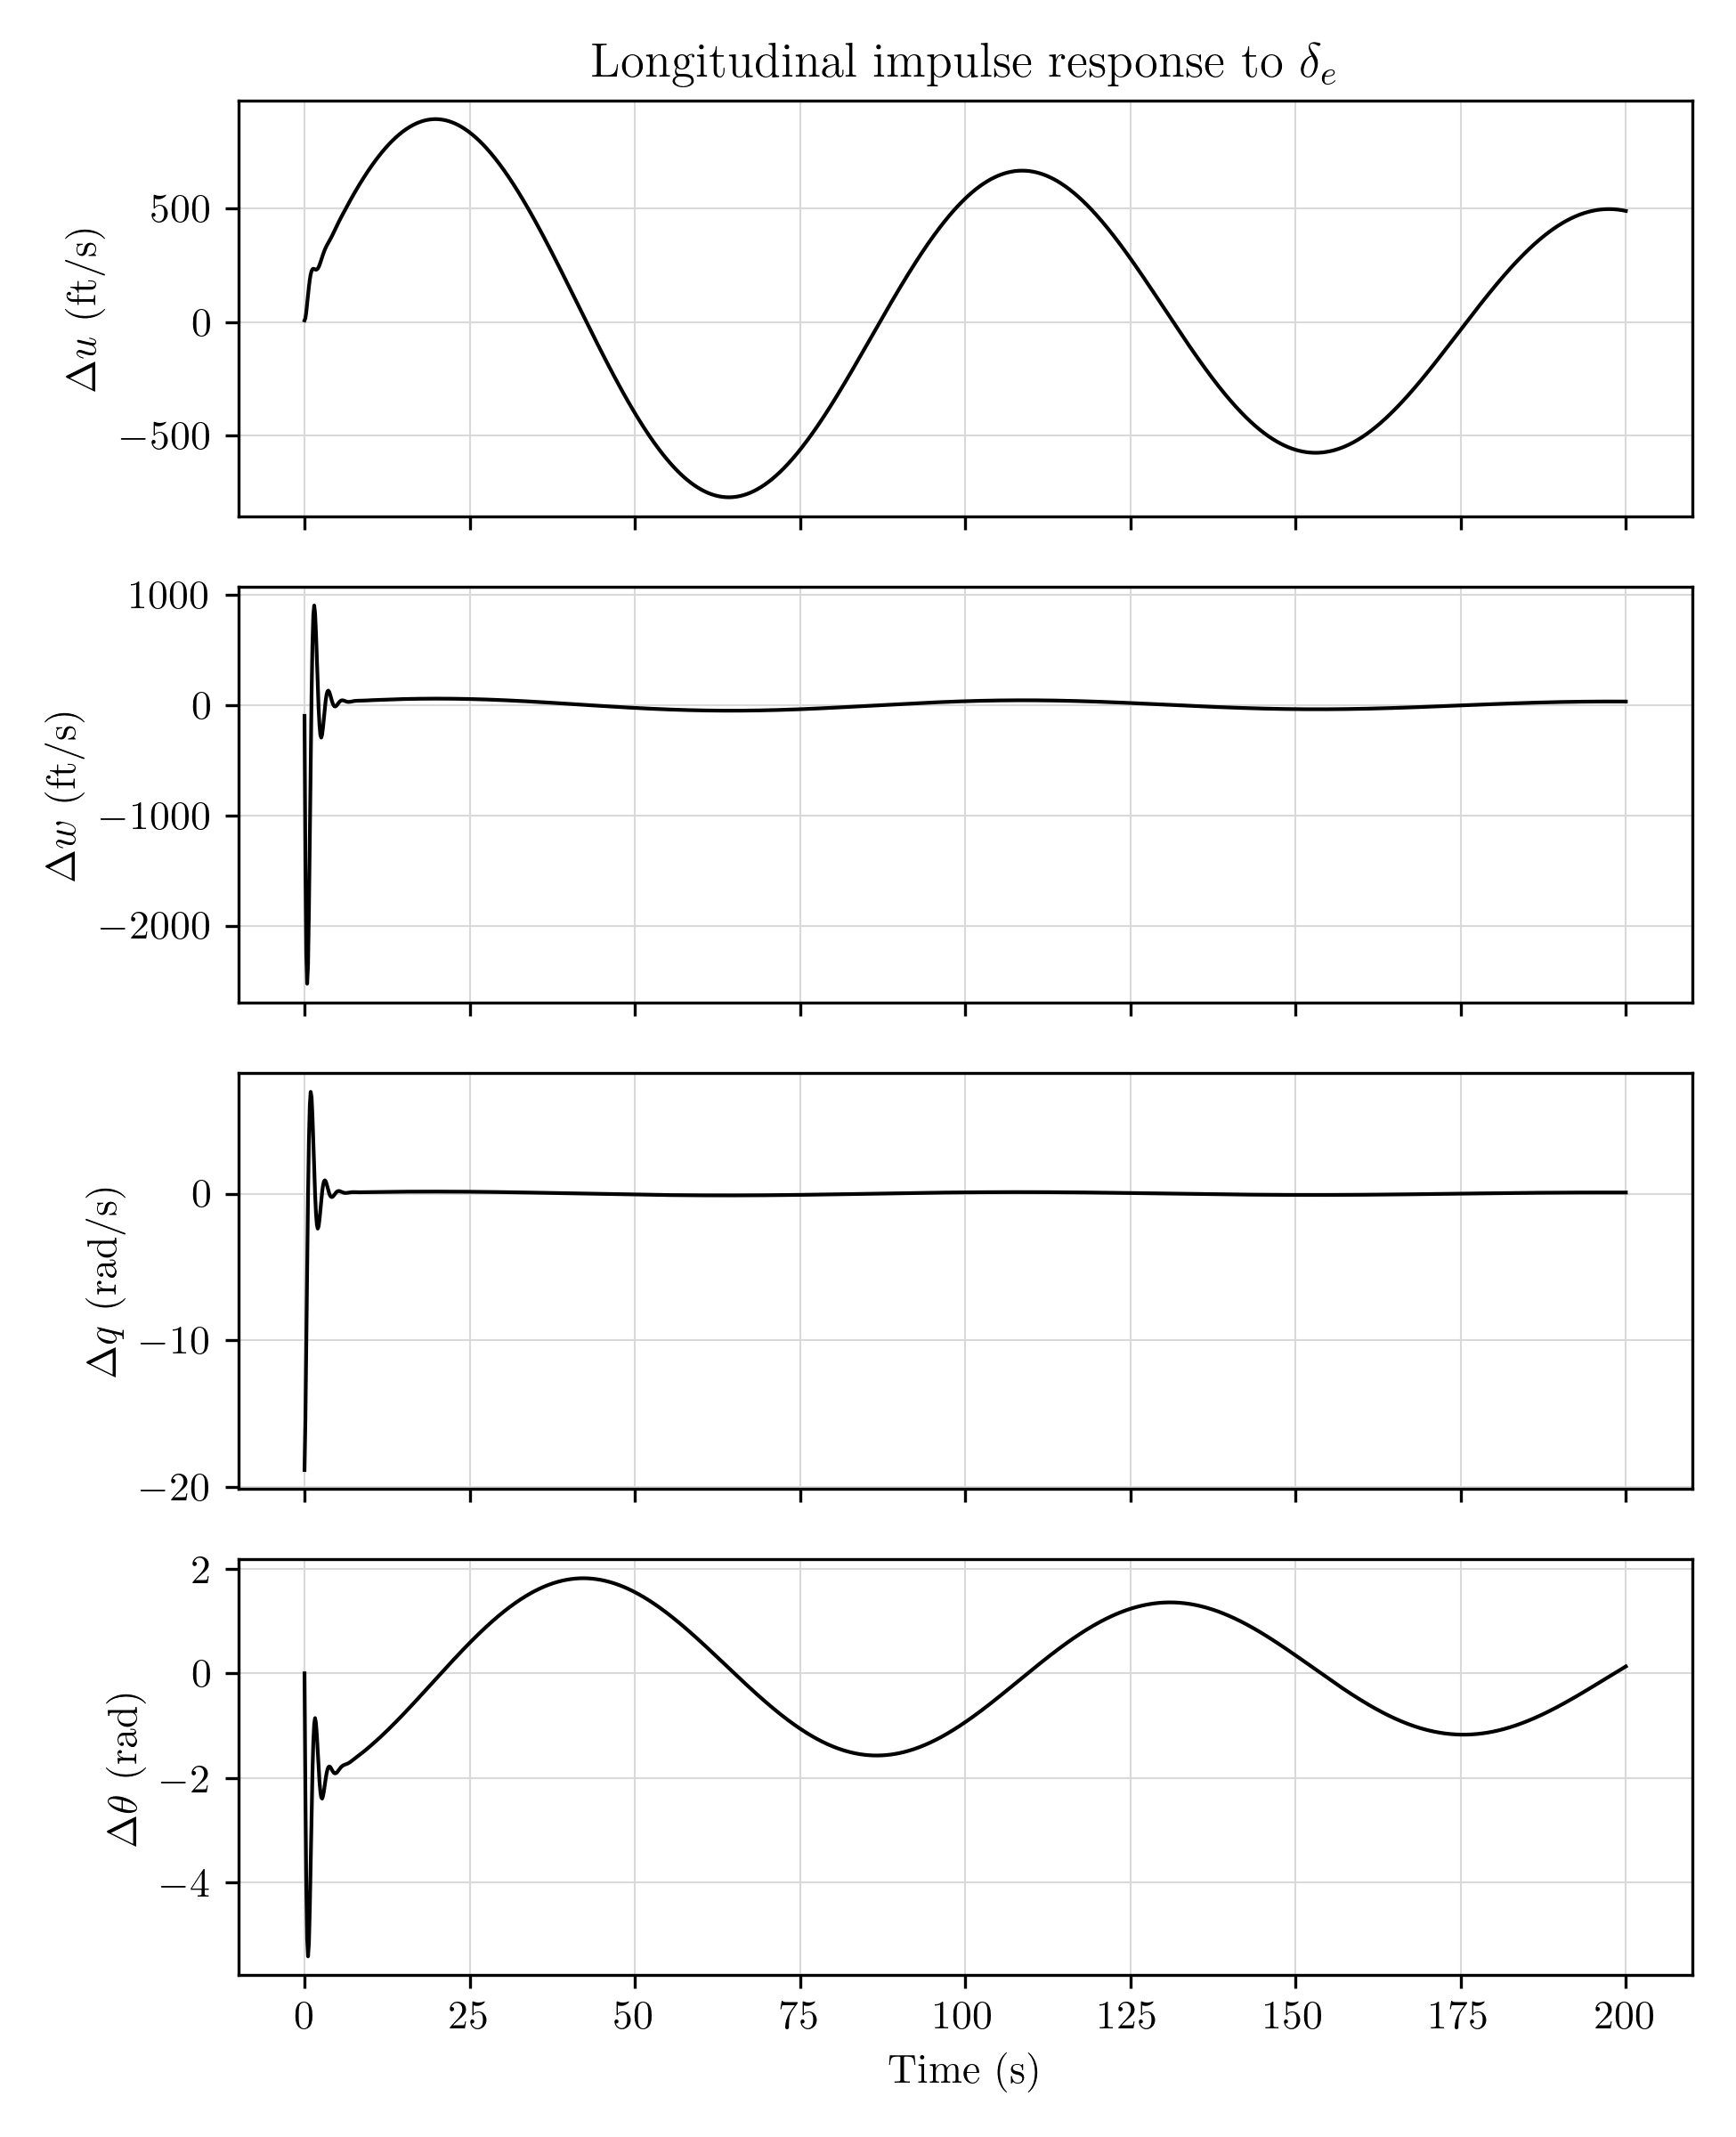
\includegraphics[width=0.78\textwidth]{figures/long_impulse_de.png}
\caption{Longitudinal impulse response to elevator deflection $\delta_e$.}
\label{fig:long-de}
\end{figure}

\begin{figure}[h]
\centering
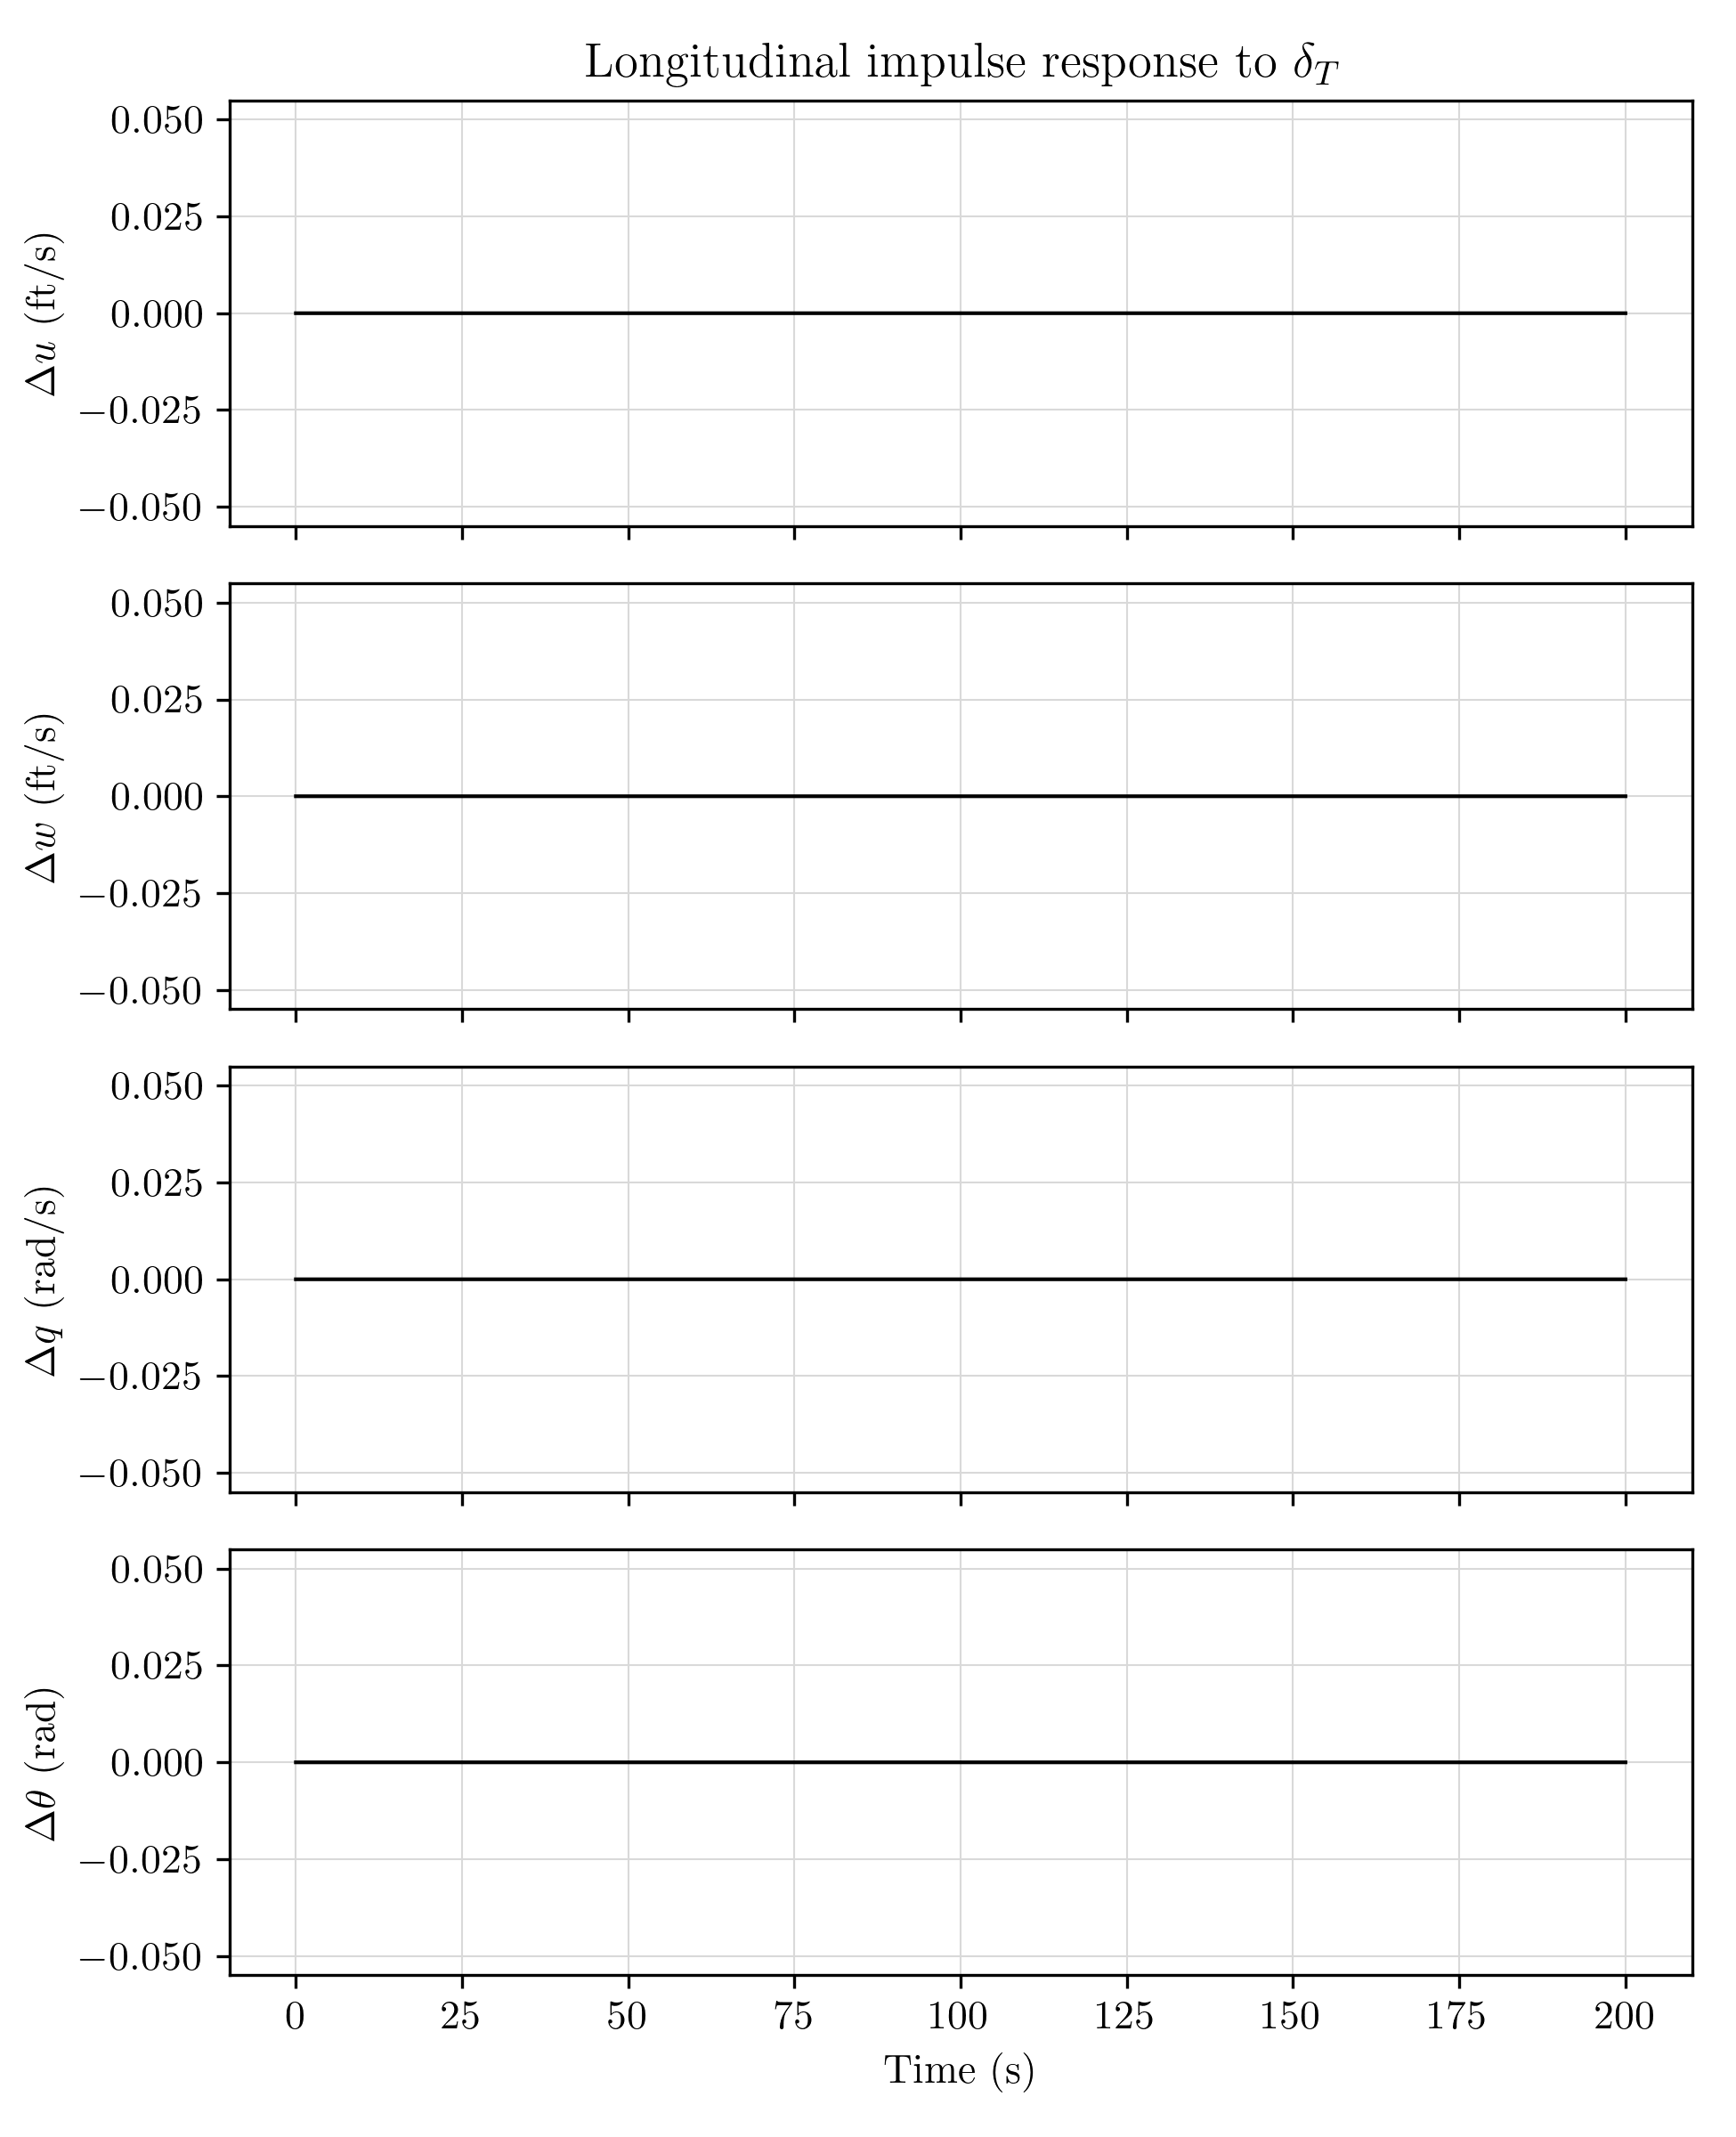
\includegraphics[width=0.78\textwidth]{figures/long_impulse_dT.png}
\caption{Longitudinal impulse response to throttle perturbation $\delta_T$.
The response is identically zero because the project handout omits throttle
derivatives, so $X_{\delta_T} = Z_{\delta_T} = M_{\delta_T} = 0$.}
\label{fig:long-dT}
\end{figure}

placeholder

\subsection{Lateral-Directional Response}

placeholder

\begin{figure}[h]
\centering
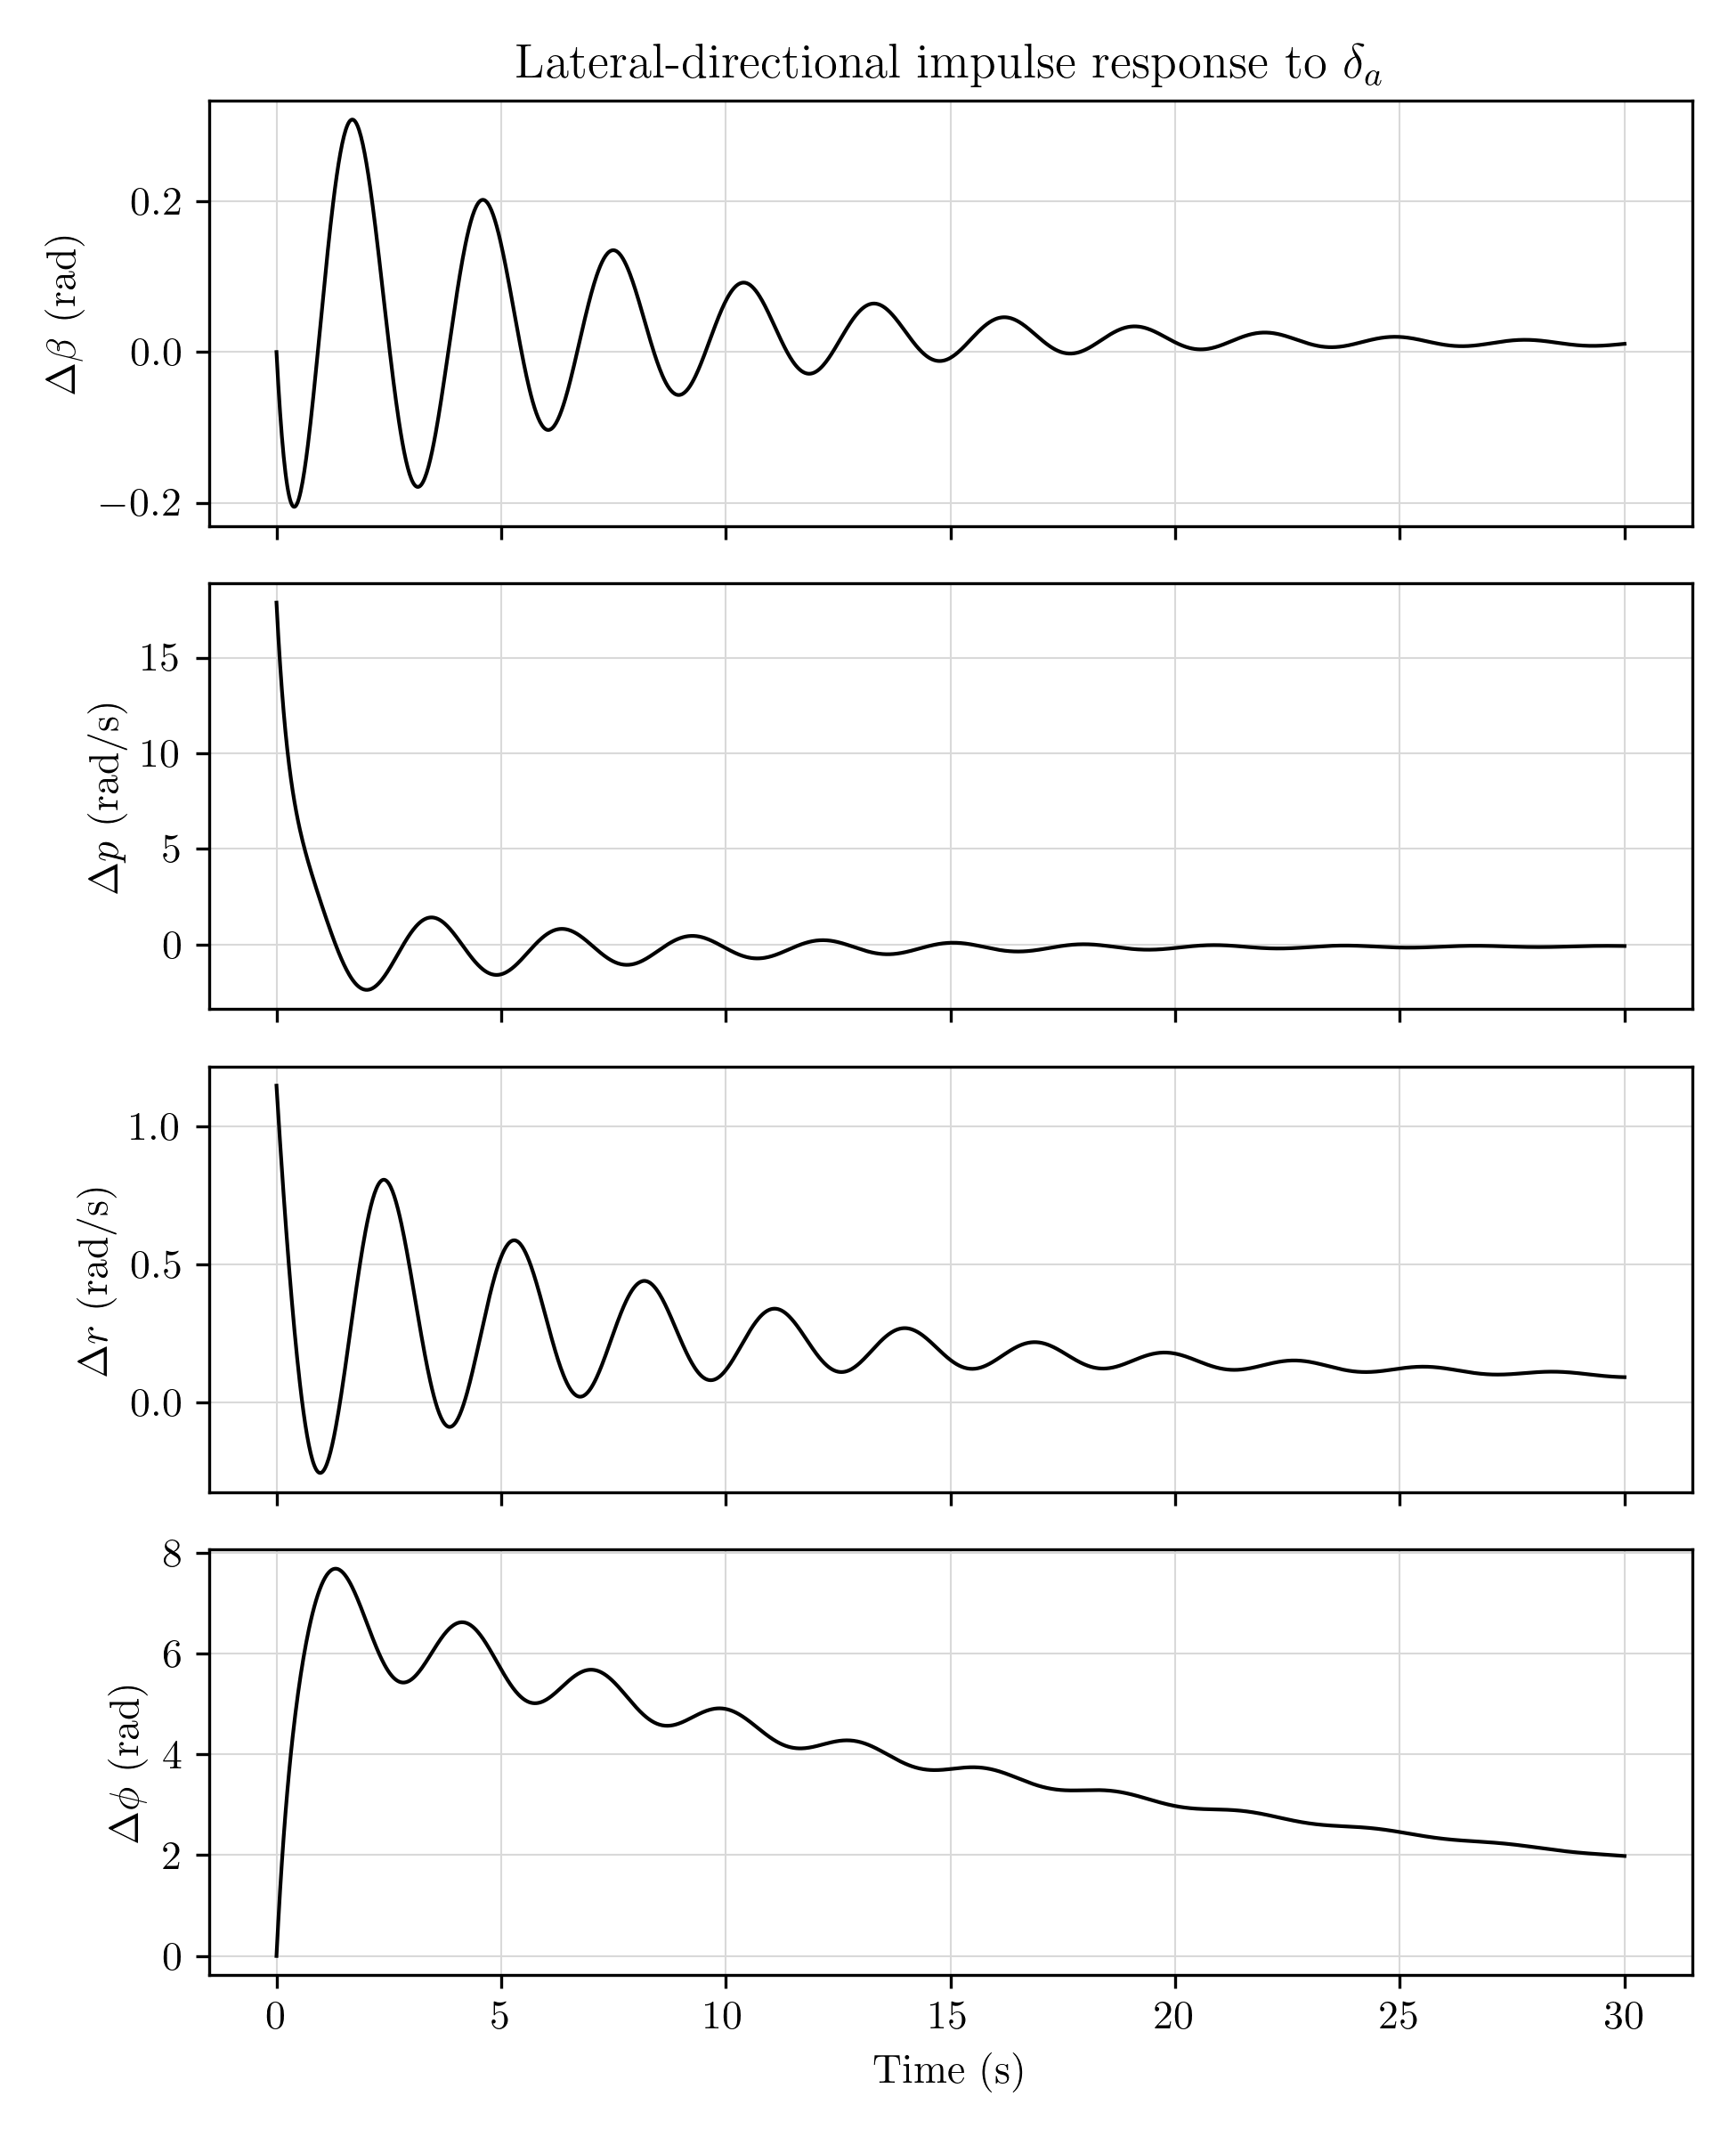
\includegraphics[width=0.78\textwidth]{figures/lat_impulse_da.png}
\caption{Lateral-directional impulse response to aileron deflection $\delta_a$.}
\label{fig:lat-da}
\end{figure}

\begin{figure}[h]
\centering
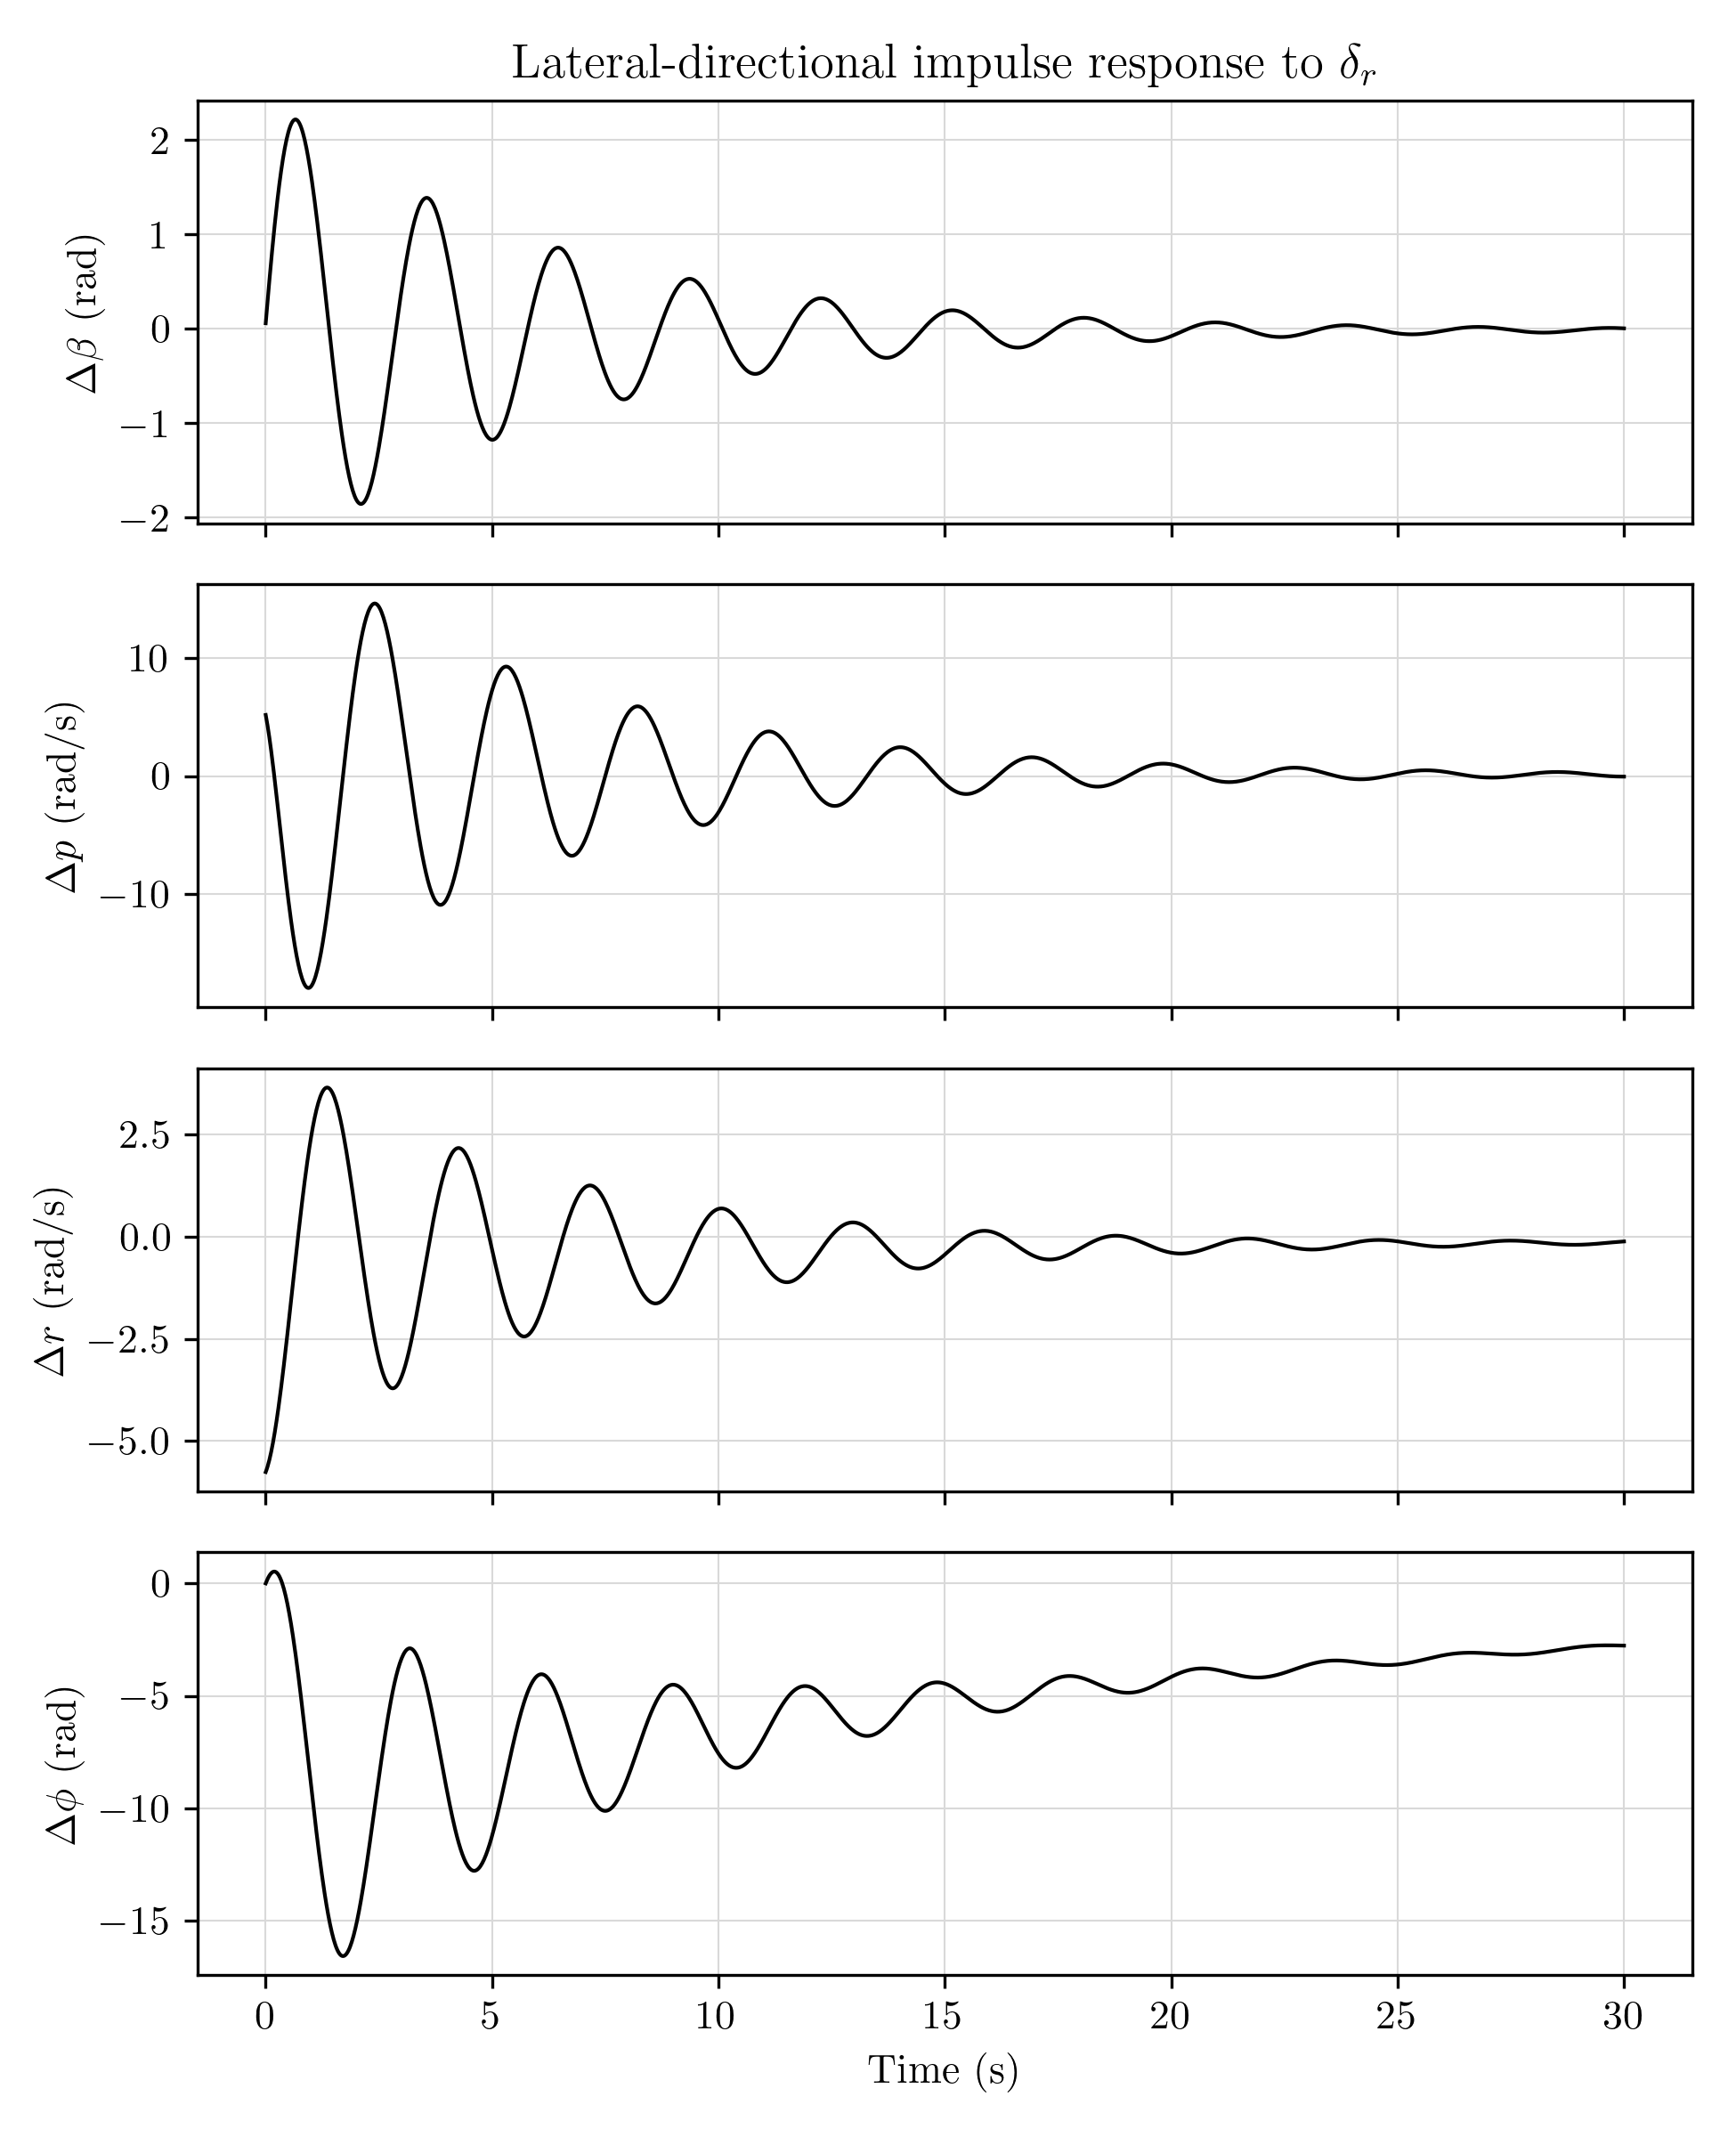
\includegraphics[width=0.78\textwidth]{figures/lat_impulse_dr.png}
\caption{Lateral-directional impulse response to rudder deflection $\delta_r$.}
\label{fig:lat-dr}
\end{figure}

placeholder

\section{Flying Qualities Assessment}

placeholder

\begin{table}[h]
\centering
\caption{MIL-F-8785C flying qualities classification (Class IV fighter,
Category B cruise).}
\begin{tabular}{l l c c}
\toprule
\textbf{Mode} & \textbf{Metric} & \textbf{Value} & \textbf{Level} \\
\midrule
Short period     & $\zeta$               & $0.316$  & Level 1 \\
Short period     & CAP (1/s$^2$)         & $0.429$  & Level 1 \\
Phugoid          & $\zeta$               & $0.0466$ & Level 1 \\
Dutch roll       & $\zeta$               & $0.0740$ & Level 2 \\
Dutch roll       & $\zeta\,\omega_n$ (1/s) & $0.161$ & --- \\
Dutch roll       & $\omega_n$ (rad/s)    & $2.171$  & --- \\
Roll subsidence  & $\tau$ (s)            & $0.334$  & Level 1 \\
Spiral           & $t_{\text{double}}$ (s) & stable & Level 1 \\
\bottomrule
\end{tabular}
\end{table}

placeholder

\appendix
\addcontentsline{toc}{part}{Appendix}

\section{Python Source Code}

The complete analysis script (\texttt{main.py}) is reproduced below. It
computes every numerical result reported above and generates all four
impulse-response figures, requiring only NumPy, SciPy, and matplotlib.

\lstinputlisting[style=pythonstyle]{main.py}

\end{document}
